\documentclass[12pt]{article}

\usepackage[utf8]{inputenc}
\usepackage[margin=1in]{geometry}
\renewcommand{\baselinestretch}{1}
\usepackage{indentfirst}

\usepackage{amsmath, amssymb}

\usepackage{hyperref}
\usepackage{cleveref}
\usepackage{graphicx}
\usepackage{float}
\graphicspath{{./figs/}}

\begin{document}

\begin{center}\begin{LARGE}
\textbf{Assignment 4: Results/Description}
\end{LARGE}\end{center}

\section*{Problem 1}

For this problem I have written three programs (\texttt{myODEInt},
\texttt{myLeapfrog}, and \texttt{myVelVerlet}) to solve the following problems.
These may be compiled all together with a \texttt{make all} as shown below.

\begin{figure}[H]
    \centering
    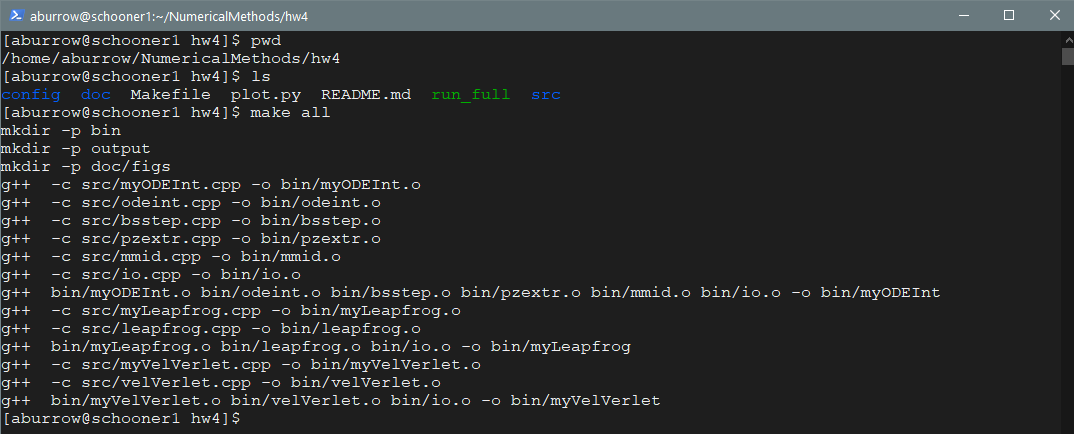
\includegraphics[width=1\textwidth]{compile}
    \label{fig:compile}
\end{figure}

This generates executables \texttt{myODEInt}, \texttt{myLeapfrog}, and
\texttt{myVelVerlet} in the ``./bin'' directory, which may be run one at a time.
There is also a \texttt{plot.py} in the root which may be run to generate plots
from the output of the executables. However, to run all these programs at once,
I have also included a \texttt{run\_full} bash script that may be executed for
convenience.

For the following problems, I am solving the second-order linear ordinary
differential equation
$$
\begin{aligned}
\frac{d^2x}{dt^2} = a(x)
\end{aligned}
$$
with acceleration $a(x) = -x$, which represents a harmonic oscillator with
$k=\omega=m=1$. This equation is solved with different methods below on the
interval $0 <= t <= 10\pi$ (5 cycles). As solution for velocity is also
simultaneously given in these methods, the kinetic energy is also given as
$T(\dot{x}) = \frac{1}{2} m\dot{x}^2 = \frac{1}{2} v^2$ (with $m=1$).

\subsection*{(a)}

Below I run the program that demonstrates solving our differential equation
using Numerical Recipes' ODE integration using the Bulirsch-Stoer method:
\begin{figure}[H]
    \centering
    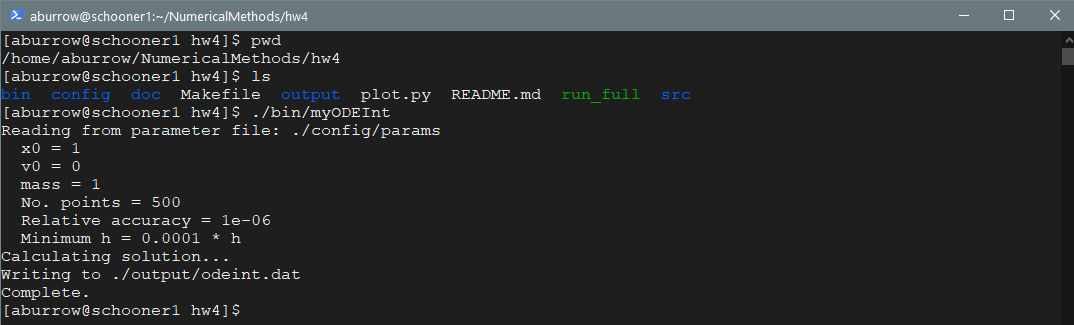
\includegraphics[width=1\textwidth]{myODEInt}
    \label{fig:myODEInt}
\end{figure}

Here I solve for 500 points of the solution, with boundary conditions $x_0 =
1$ (initial position) and $v_0 = 0$ (initial velocity). The position solution
is plotted in the left panel of \autoref{fig:odeint}, and the kinetic energy of
the system is plotted in the right panel. The residuals are also given below
each panel. For this solution, we see that the calculated solution compares
very well with the expected analytic solution $x(t) = x_0 \cos t$. The
residuals show that it fits the solution on order of $10^{-11}$, which is
similar to what we found in Assignment 3. A similar result is found for the
energy.

\begin{figure}[ht]
    \centering
    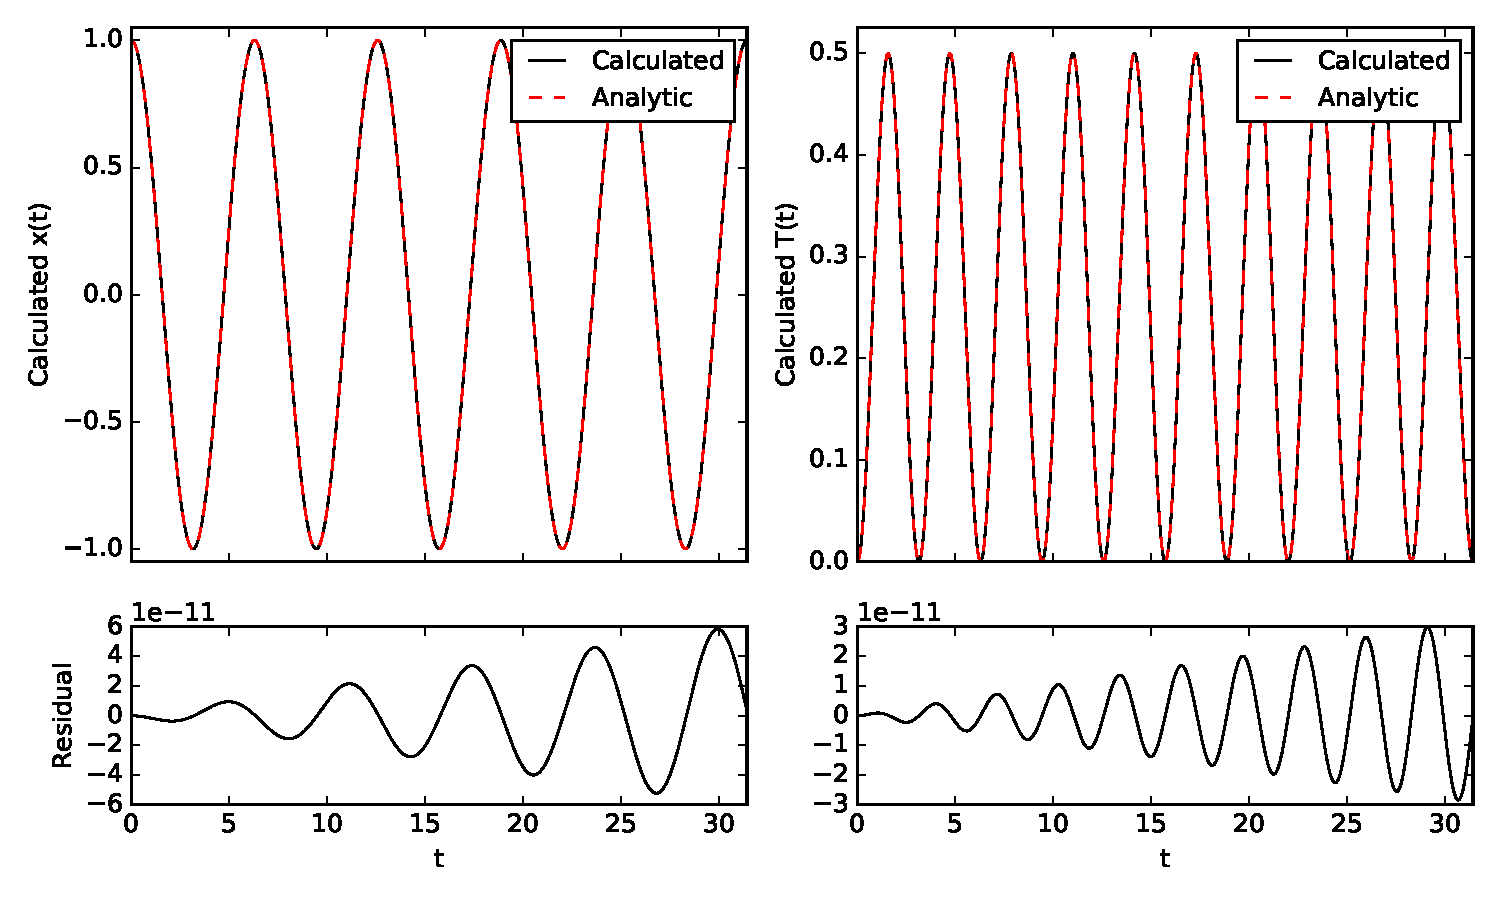
\includegraphics[width=0.9\textwidth]{odeint}
    \caption{Solution using the ODEInt (BS) method. Left panel: Position vs.
             time; right panel: Kinetic energy vs. time.}
    \label{fig:odeint}
\end{figure}

Interestingly, it seems that the residuals tend to increase as a function of
time between the maxima and minima.

\subsection*{(b)}

Below I run the program that demonstrates solving the differential equation
using the Leapfrog method, the algorithm for which was given to us in the
assignment problem:
\begin{figure}[H]
    \centering
    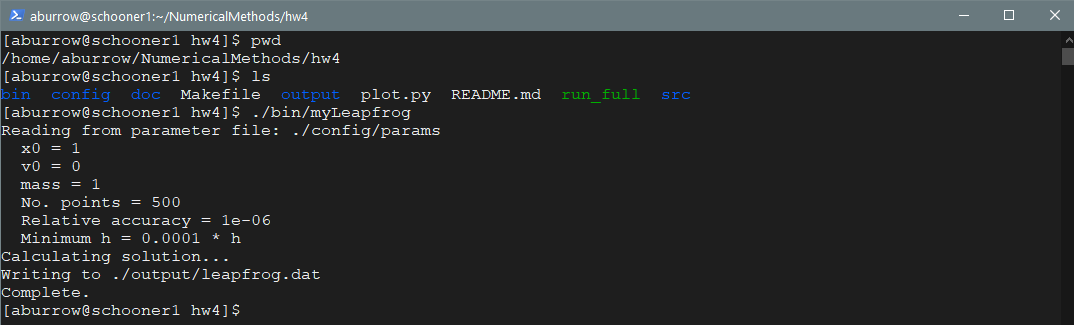
\includegraphics[width=1\textwidth]{myLeapfrog}
    \label{fig:myLeapfrog}
\end{figure}

Here I calculate the solution at the same 500 points with the same boundary
conditions. The corresponding position and kinetic energy plot is displayed in
\autoref{fig:leapfrog}. We see that the solution is again fitting of the
analytic solution, however this time this method produces residuals on order of
$10^{-3}$, and therefore it appears to be a weaker solution. And yet again, we
see the residuals increase as a function of time.

\begin{figure}[ht]
    \centering
    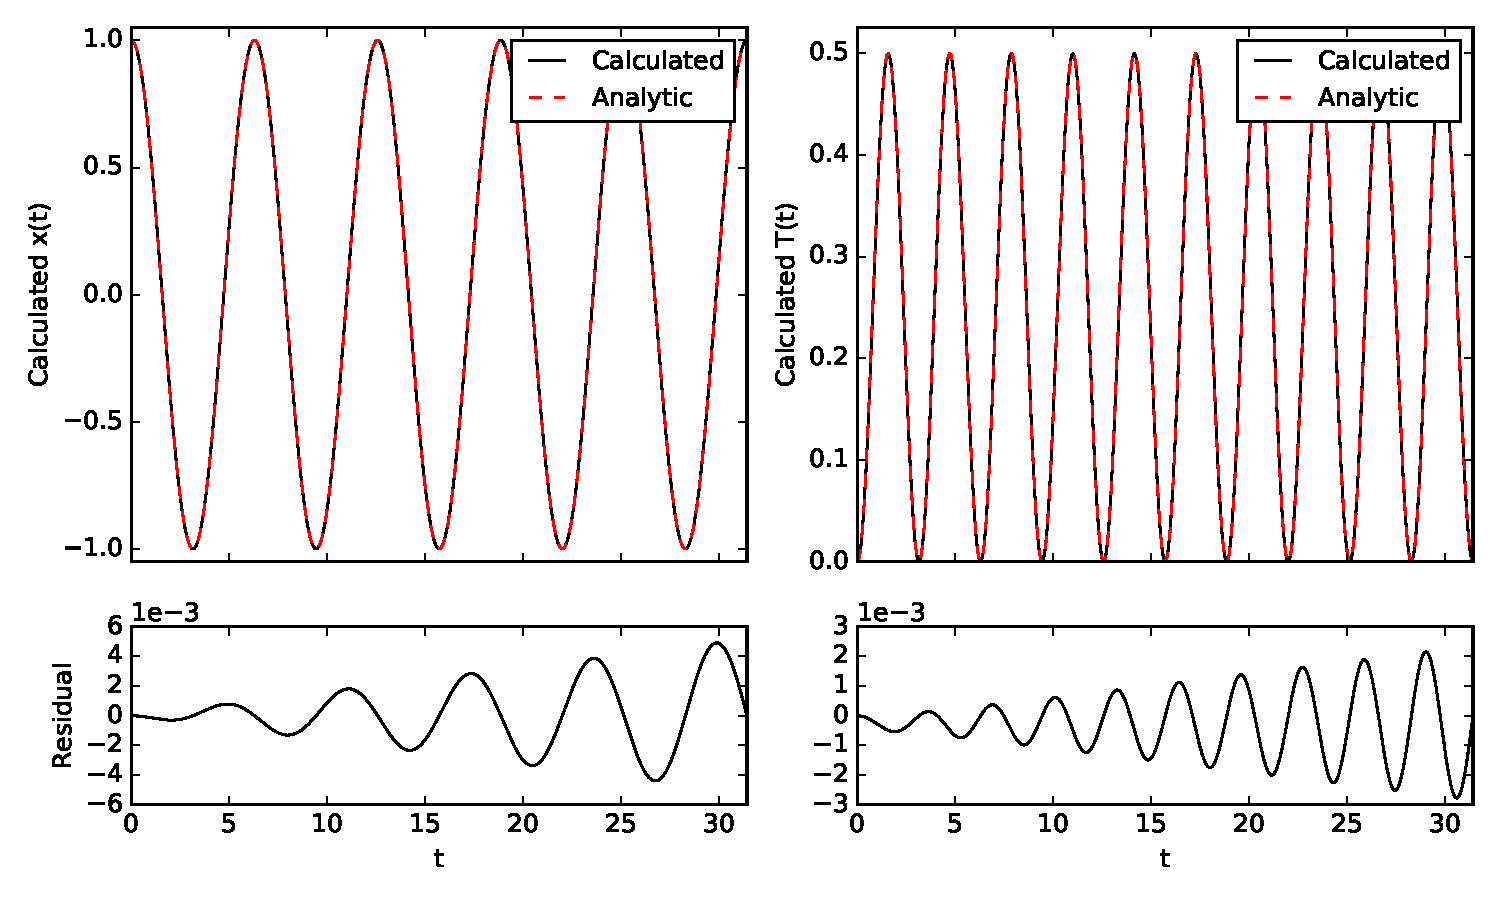
\includegraphics[width=0.9\textwidth]{leapfrog}
    \caption{Solution using the Leapfrog method. Left panel: Position vs.
             time; right panel: Kinetic energy vs. time.}
    \label{fig:leapfrog}
\end{figure}

\subsection*{(c)}

Below I run the program that demonstrates solving the differential equation
using the Velocity Verlet method, the algorithm for which was given to us in
the assignment problem:
\begin{figure}[H]
    \centering
    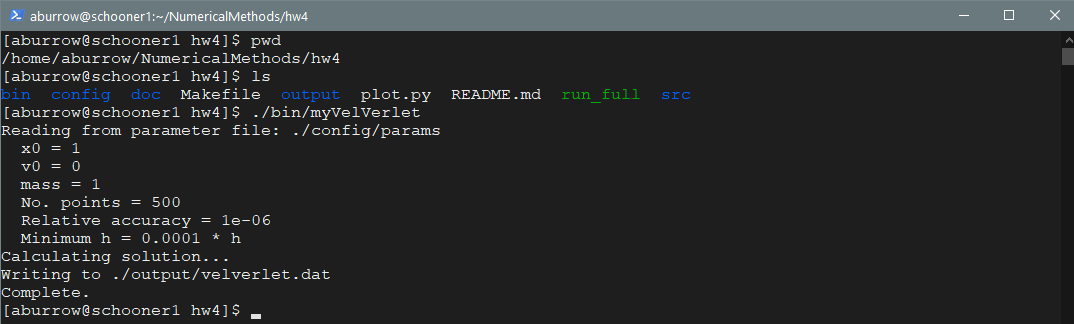
\includegraphics[width=1\textwidth]{myVelVerlet}
    \label{fig:myVelVerlet}
\end{figure}

This algorithm is just the same as the Leapfrog method in this case. With $m=1$,
the code itself could be the exact same (where $F \rightarrow a$ and
$p \rightarrow v$). However, I developed my code for this case to be more
generalized just to compare and contrast the results. This is done with a
force function that the user provides (it is in the myVelVerlet.cpp file).

I calculate again at the same 500 points with the same boundary conditions. The
corresponding position and kinetic energy plot is in \autoref{fig:velverlet}.
From the plot, it is apparent that the result is the exact same one as the
leapfrog method (see \autoref{fig:leapfrog}). However, in reality something in
my code must have altered the results very slighty. Looking at the position
column of the raw output, the last few digits of precision begin to deviate
from those in the leapfrog solution over time $t$. This would likely be caused
by the introduction of mass and the divisions necessary to transform from
momentum/force to velocity/acceleration.

\begin{figure}[ht]
    \centering
    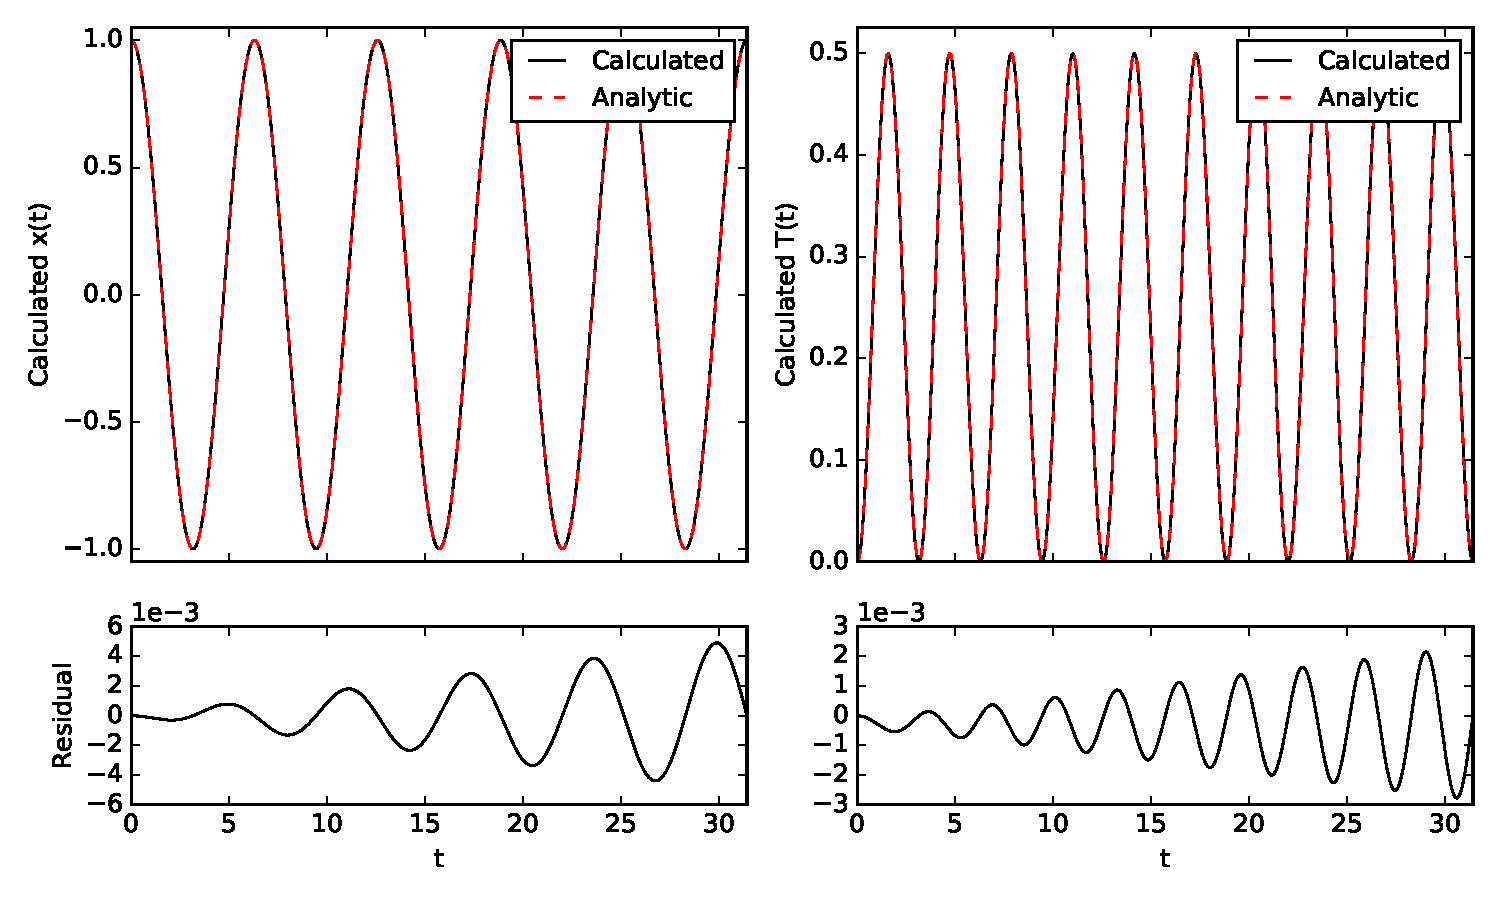
\includegraphics[width=0.9\textwidth]{velverlet}
    \caption{Solution using the Velocity Verlet method. Left panel: Position
             vs. time; right panel: Kinetic energy vs. time.}
    \label{fig:velverlet}
\end{figure}

\subsection*{(d)}

Looking at the plots, all three methods seem to do a fairly good job at
calculating the solution to this differential equation, especially given the
ease that the latter two methods took to code and perform. However, it is again
abundantly clear that the Bulirsh-Stoer method is superior in calculating the
solution by several orders of magnitude.

As stated before, it is also clear that Leapfrog and Velocity Verlet methods
are effectively the same, however care must be taken when performing extra
calculations (divisions, subtractions, etc.) to ensure the accuracy of the last
few digits of precision in the values we get from them.


\end{document}
